\chapter{Anexos}

\section{Glosario}

\textbf{.txt}: El .txt es el formato de los documentos de texto plano.

\textbf{Algoritmo}: Un algoritmo se define como un conjunto de ordenes definidas y finitas con el objetivo de llegar a una solución a un problema, la realización de un computo, proceso de datos u otras actividades. El estudio de los algoritmos busca una constante mejora de la resolución de problemas empleando métodos distintos, con el fin de optimizar los recursos necesarios, así como una solución estandarizada y apropiada para un problema general.

\textbf{API}: Una API es una Interfaz de Programación de Aplicaciones, es un conjunto de protocolos y definiciones empleada en el desarrollo e integración de Software que se emplea como una biblioteca.

\textbf{Animación}: La animación es el acto de producir imágenes en movimiento; técnica que significa que provee de movimiento a una grabación o una serie de dibujos (Oxford English Dictionary). 

\textbf{Código}: El código en el contexto, se define como el conjunto de símbolos y signos que se transmiten de un emisor a un receptor, cuya intención es privar del conocimiento de su contenido a terceros. Un código tiene un conjunto de reglas o normas que se emplean para dificultar la lectura del mensaje, siendo un ejemplo la traducción de un mensaje en español a ingles, el mensaje puede ser solo entendido por quien conozca el idioma ingles.

\textbf{Cmake}: Es una herramienta multiplataforma de automatización o generación de código, abreviatura de "cross platform make".

\textbf{CUDA}: Sigla de Compute Unified Device Architecture, se emplea para referenciar una plataforma de computación en paralelo, con compilador y herramientas de desarrollo creado por nVidia.

\textbf{Dataset}: Un dataset es una tabla dentro de una base de datos, en la cual se representa una variable particular en la primera columna, y cada fila es un componente del conjunto de datos.

\textbf{Decodificador}: El decodificador es una herramienta que permite descifrar un mensaje codificado. Se refiere a la actividad inversa de la codificación, implica la recepción de un código y de acuerdo al conjunto de normas establecidas para su traducción, se lo interpreta y se obtiene el mensaje inicial que se deseaba recibir.

\textbf{Frame}: Las grabaciones o serie de dibujos están compuestas por cuadros o Frames en ingles, que son una imagen individual de la secuencia de imágenes que componen la animación para dar la sensación de movimiento. La mayoría de las animaciones emplean de 24 a 30 Frames per second (FPS). 

\textbf{Framework}: El Framework es toda estructura conceptual y tecnológica de soporte definido, con artefactos o módulos de Software que sirven para la el desarrollo y organización de Software.

\textbf{Hardware}: El Hardware se entiende como el componente físico de una computadora o dispositivos de Von Neumann. Esta compuesto por el procesador, la tarjeta madre, RAM, disco duro, monitor, dispositivos de entrada y salida, los cuales normalmente se mencionan como componentes y a los dispositivos externos como periféricos\cite{hardwaredef}.

\textbf{GPU}: La unidad de procesamiento gráfico (GPU o Graphics processing unit) es un procesador suplementario al  central, aligera la carga para trabajar con gráficos u operaciones de tipo flotante, normalmente usado en aplicaciones 3D interactivas. 

\textbf{GUI}: Una interfaz gráfica de usuario (Graphical user interface o GUI) es una interfaz diseñada con imágenes y gráficos para la representación de la información y controles disponibles en la interfaz del usuario.

\textbf{UI}: La interfaz puede ser usada tanto en un contexto de Hardware o de usuario, siendo la segunda la definición relevante.
Una interfaz de usuario (UI) tiene la función de otorgar al usuario el control de una aplicación de Software o un dispositivo de Hardware. Uno de los objetivos de la UI es ser amigable con el usuario, permitiendo interactuar con la aplicación de manera intuitiva y natural. Ejemplos de UI pueden ser la pantalla de inicio de una pagina web y de Hardware un control remoto de televisión.

\textbf{JPG}: Es un formato estándar de codificación y compresión de imágenes y archivos estáticas. JPG es una abreviación de Joint Photographic Experts Group (JPEG), comité que creo dicho formato.

\textbf{JSON}: El JavaScript Object Notation es un formato ligero e independiente de lenguajes para la transmisión de datos, es de simple lectura y fácil para el procesamiento de la máquina.

\textbf{Software}:El software esta construido para ejecutar dispositivos von Neumann multiproposito. Un software contienen secuencias de declaraciones de programas abstractos que describen las tareas que deben ser realizadas por una maquina. 

\textbf{Modelo de Von Neumann}: Es una arquitectura de computadoras, su objetivo es explicar como funciona una computadora y la interacción entre sus distintos componentes (CPU, ALU, RAM y otros).

\textbf{Interprete}:El interprete en el contexto informático es un programa traductor que permite ejecutar otros programas a lenguaje máquina, a diferencia de los compiladores, estos solo ejecutan la sección que requieren emplear.

\textbf{Pixel}: El pixel es la unidad mínima homogénea en color que en su conjunto da forma a una imagen digital.

\textbf{Plug-in}: Un plugin o complemento es un Software o Aplicación con un grupo de características y funciones especificas para interactuar por medio de una API.

\textbf{Shell}: Shell es un interprete de comandos para acceder y emplear los servicios del sistema operativo, son necesarios para ejecutar los programas de una computadora.

\textbf{Script}: El script es una secuencia de comandos, estos son ejecutados primero por un interprete que lee el codigo fuente o una consola interactiva para que el usuario trabaje. Se los utiliza para automatizar tareas repetitivas, interactuar con el sistema operativo y otros.

\textbf{SDK}: El kit de desarrollo de Software (Software development kit o SDK) es un conjunto de herramientas para el desarrollo de Software, permite la creación de una aplicación para sistemas concretos, es una API creada para poder usar ciertos lenguajes de programación y en algunos casos, comunicarse con ciertos sistemas embebidos, en algunos casos, son capaces de detectar errores y aportar utilidades extra.

\section{Proceso de Instalación de OpenPose y Unity para el Desarrollo del Proyecto}

Inicialmente se deben instalar la SDK de Visual Studio 2019 , de la pagina oficial  \href{https://visualstudio.microsoft.com/es/thank-you-downloading-visual-studio/?sku=Community&rel=16}{visualstudio.microsoft.com}, se ejecuta el archivo, se selecciona el paquete de idioma deseado y se lo descarga.

Posteriormente, se debe seleccionar la versión deseada, en este caso se trabajo con "Visual Studio Community 2019", se deben habilitar las opciones prrincipales de "Desarrollo de .NET", "Desarrollo para el escritorio con C++", "Desarrollo de juego con Unity", para realizar este proyecto. Se tiene que habilitar todas las opciones relacionadas con C++ y las Build Tools VS 2015-2017 en "Desarrollo para el escritorio con C++" como se observa en la figura \ref{vsinstall} de la sección de anexos, ya que OpenPose las utiliza, finalmente se lo debe instalar en el lugar deseado y ejecutar.

La instalación de Unity inicia vistiando su pagina oficial de descargas  \href{https://unity3d.com/es/get-unity/download}{unity3d.com/es/get-unity/download}, se selecciona la opción de Descarga Unity Hub, se selecciono la opción "Personal" y de "Usuario recurrente", finalmente se aceptan los términos y condiciones, para descargar el instalador, se lo ejecutara y configurara como se desee, se debe ejecutar el programa instalado "Unity Hub".  

En la página oficial de versiones existentes \href{https://unity3d.com/get-unity/download/archive}{unity3d.com/get-unity/download/archive}, se seleccionara la versión Unity 2019.4.14 y se selecciona la opción "Unity Hub", finalmente se acepta instalar la versión correcta, si se siguieron correctamente los pasos, se tendrá la instalación de la figura \ref{installunity} de la sección de anexos al finalizar.

La herramienta de Body Tracking OpenPose tiene requisitos elevados para su instalación y desarrollo, si bien instalar el programa para modificar el código fuente original puede realizarse siguiendo las instrucciones de  \href{https://github.com/CMU-Perceptual-Computing-Lab/openpose/blob/master/doc/installation/README.md}{openpose/doc/installation/README.md} guardado en el repositorio principal de GitHub (CMU-Perceptual-Computing-Lab/openpose). Sin embargo, se empleara su plug-in de Unity almacenado en el repositorio  \href{https://github.com/CMU-Perceptual-Computing-Lab/openpose\_unity\_plugin}{CMU-Perceptual-Computing-Lab/openpose\_unity\_plugin} de GitHub.
Se deben realizar x pasos para instalarlo, básicamente seguir las instrucciones de su documentación de instalación. Primero descargar el repositorio de GitHub, ejecutar el archivo "getPlugins.bat", "getModels.bat" y "testBinary.bat" dentro de la carpeta, para descargar los modelos, los archivos binarios de OpenPose y una demo con la cual realizar pruebas. Finalmente se abre la escena "Demo.Unity" localizada en ./OpenPosePlugin/Assets/OpenPose/Examples/Scenes/ en Unity y ejecutarla, si se realizaron todos los paso correctamente, se le pedirán aceptar dos problemas debido al versionamiento y será dirigido a la siguiente pantalla de Unity de la figura \ref{unitydemo} de la sección de anexos. 

\section{Sección de gráficos anexados}


\begin{figure}[b!]
	\centering
	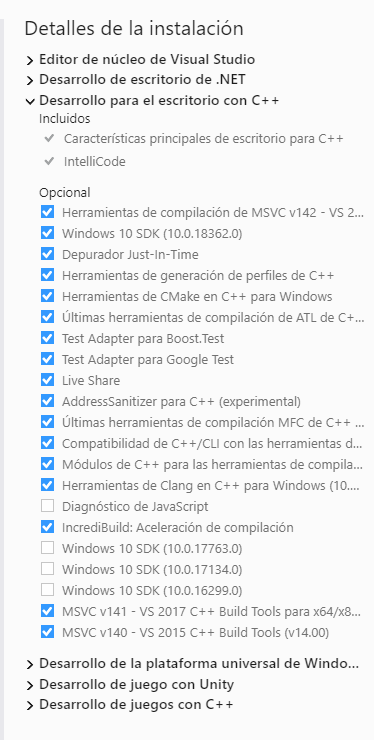
\includegraphics[width=11cm,height=18cm,]{./Images/eleccionesvsinstall.png}
	\caption{Elección Personal del Estudiante para Configurar Visual Studio 2019}
	\footnotesize Fuente: Instalador de Visual Studio.
	\label{vsinstall}
\end{figure}


\begin{figure}[t!]
	\centering
	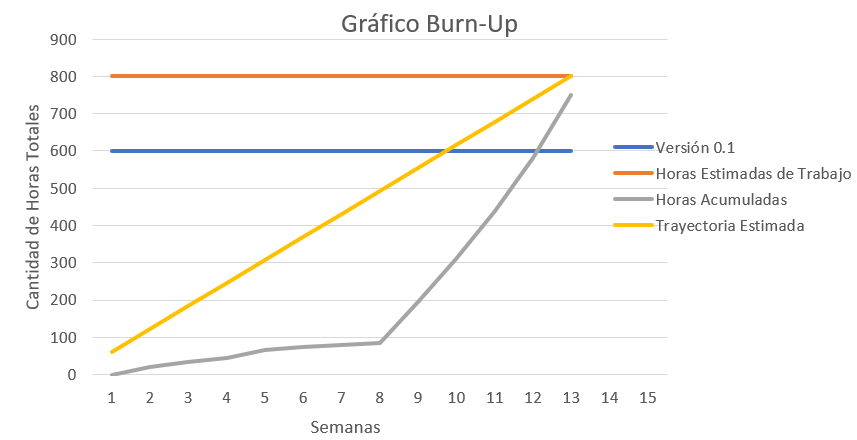
\includegraphics[width=14cm,height=8cm,]{./Images/graficoburnup.png}
	\caption{Gráfico Burn-Up}
	\footnotesize Fuente: Elaboración Propia
	\label{burnup}
\end{figure}

\begin{figure}[t!]
	\centering
	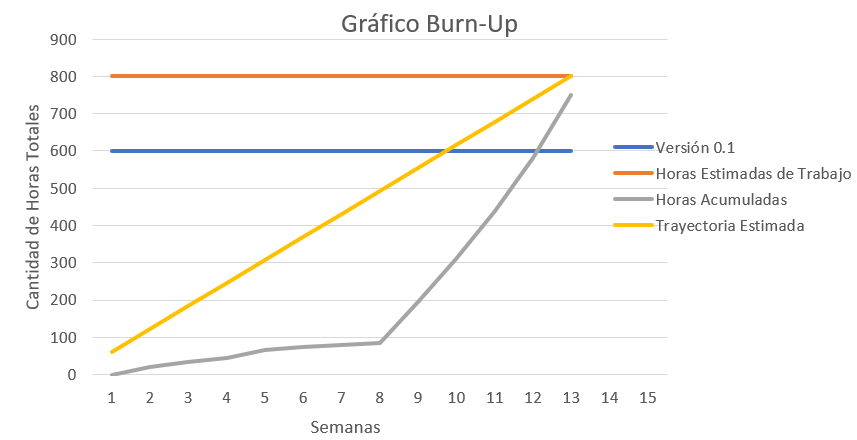
\includegraphics[width=14cm,height=8cm,]{./Images/graficoburnup.png}
	\caption{Gráfico Burn-Down}
	\footnotesize Fuente: Elaboración Propia
	\label{burndown}
\end{figure}

\begin{figure}[t!]
	\centering
	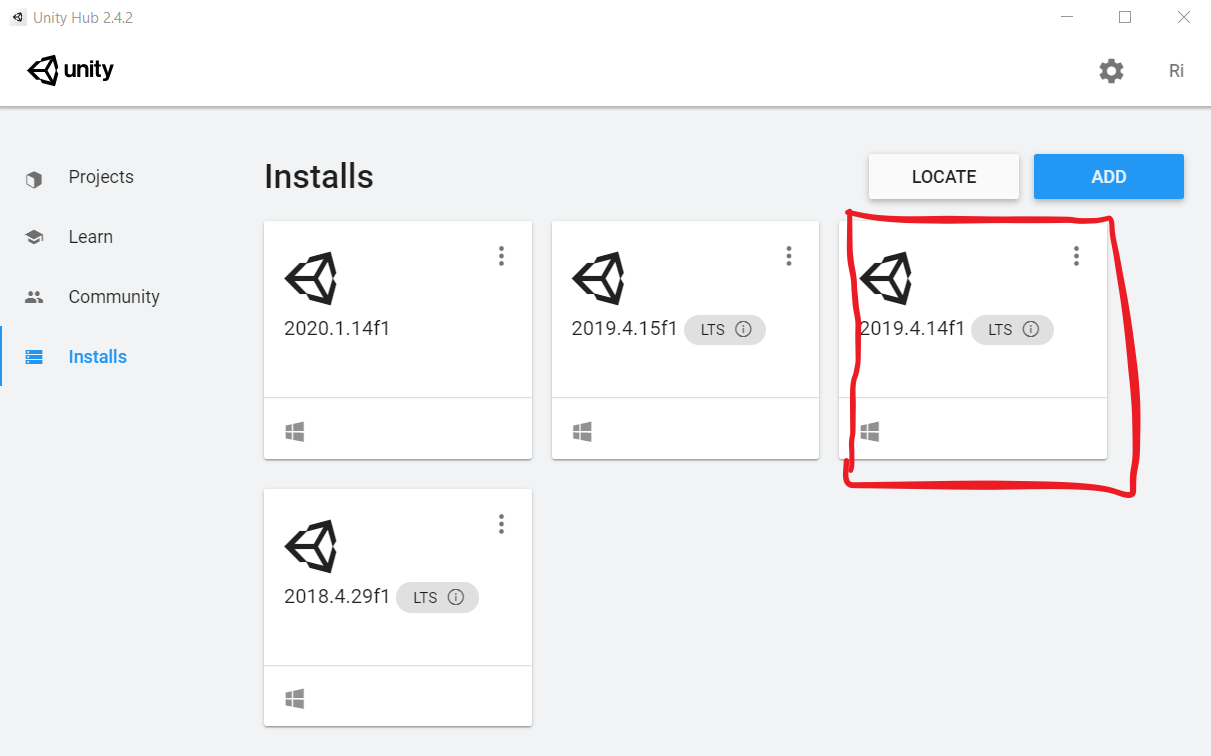
\includegraphics[width=14cm,height=10cm,]{./Images/installunity.png}
	\caption{Version Deseada de Unity Encerrada en Rojo}
	\footnotesize Fuente: Captura de Pantalla de Installs de Unity Hub.
	\label{installunity}
\end{figure}

\begin{figure}[t!]
	\centering
	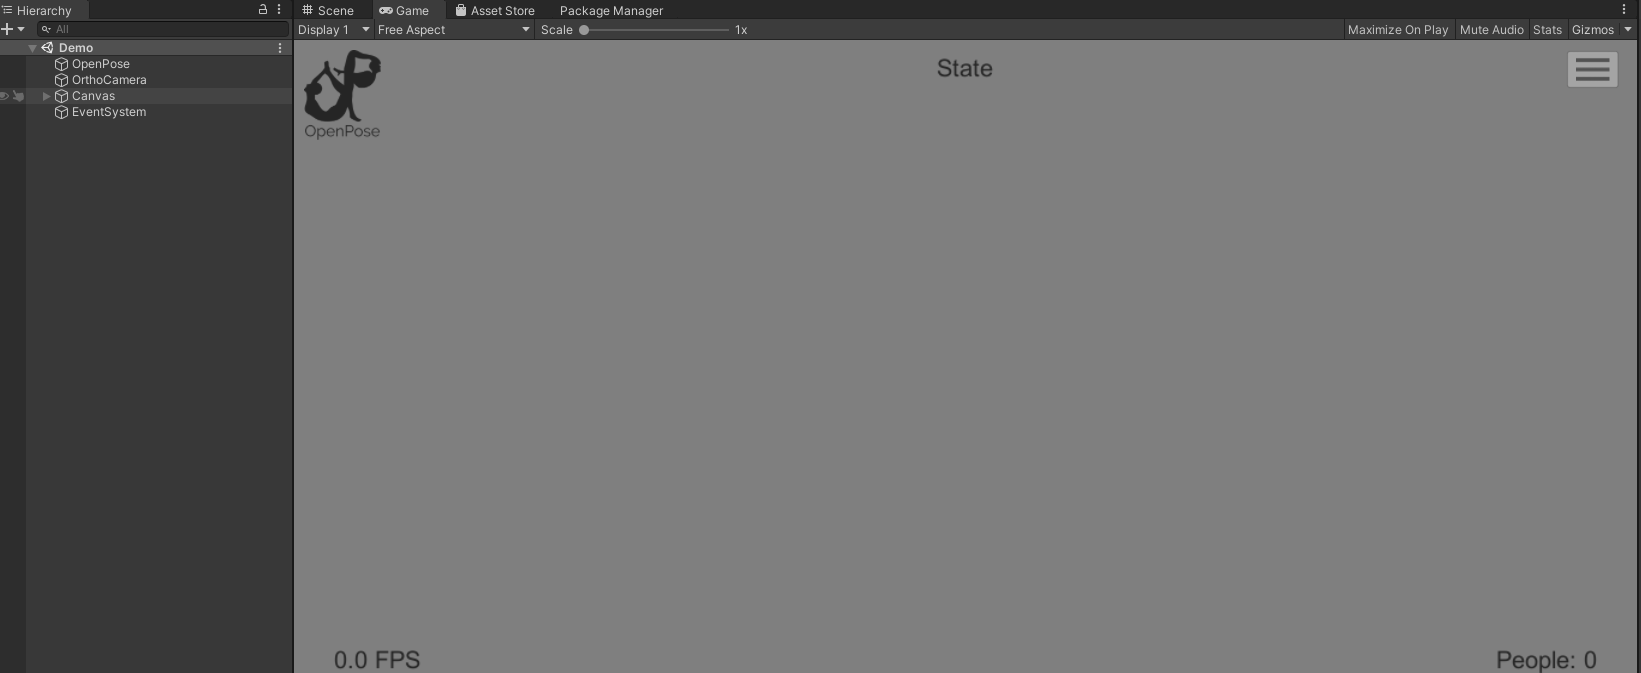
\includegraphics[width=14cm,height=7cm,]{./Images/unitydemo.png}
	\caption{Captura de Pantalla de la Configuración Inicial de OpenPose Plug-in}
	\footnotesize Fuente: \cite{8765346}\cite{cao2017realtime}\cite{simon2017hand}\cite{wei2016cpm}
	\label{unitydemo}
\end{figure}

\begin{landscape}

\begin{figure}[t!]
	\centering
	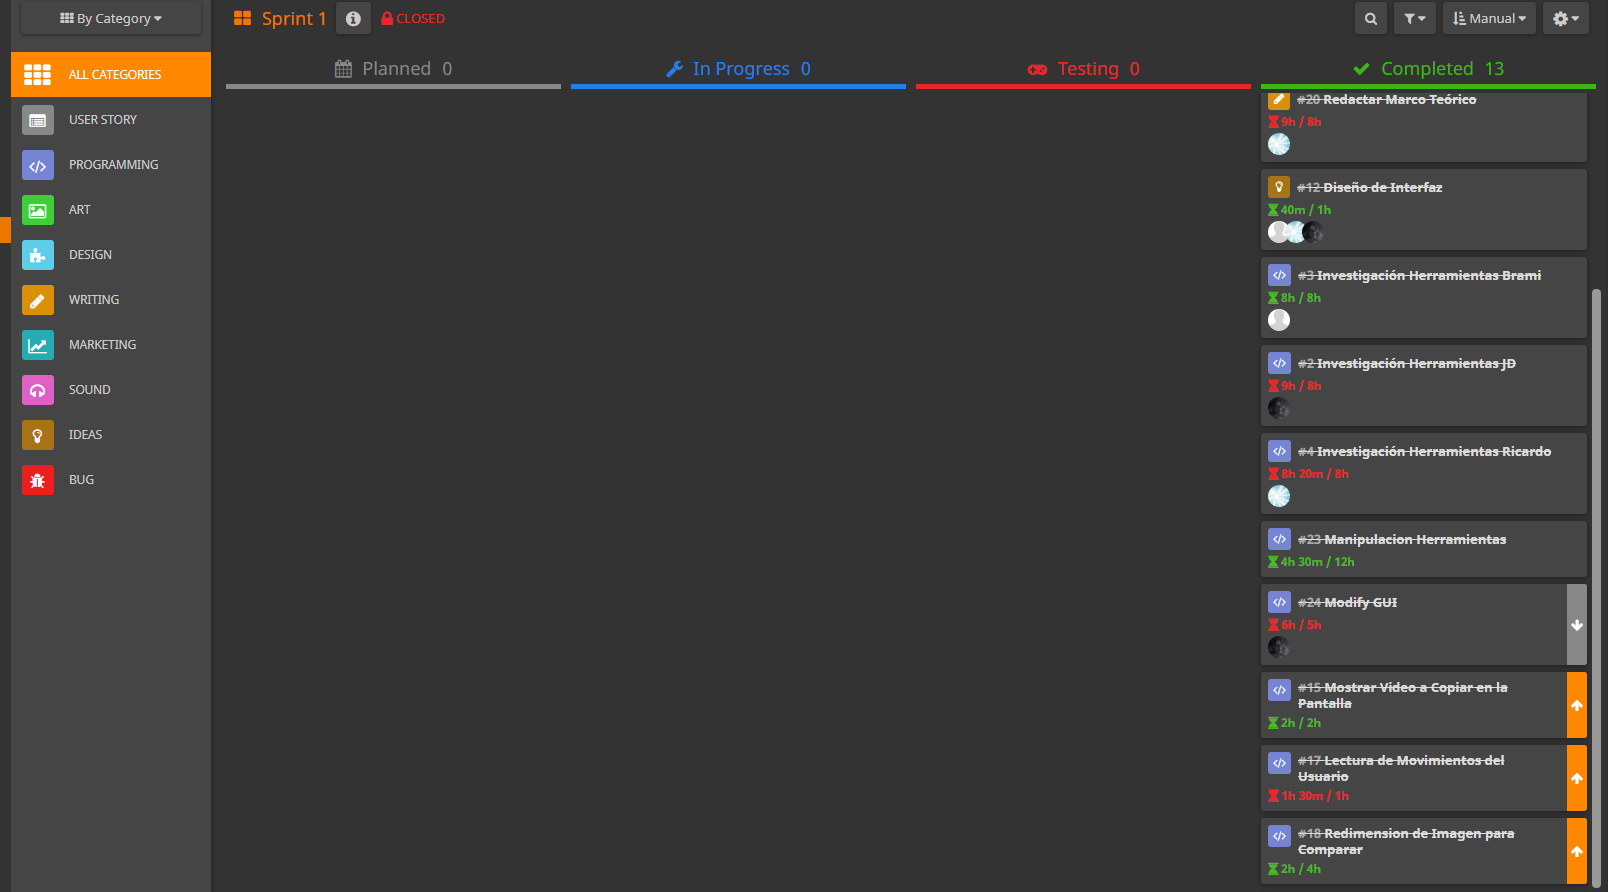
\includegraphics[width=23cm,height=15cm,]{./Images/sprintexample2.png}
	\caption{Sprint 1 concluida}
	\footnotesize Fuente: Elaboración Propia empleando la herramienta HacknPlan.
	\label{sprintexample2}
\end{figure}

\begin{figure}[t!]
	\centering
	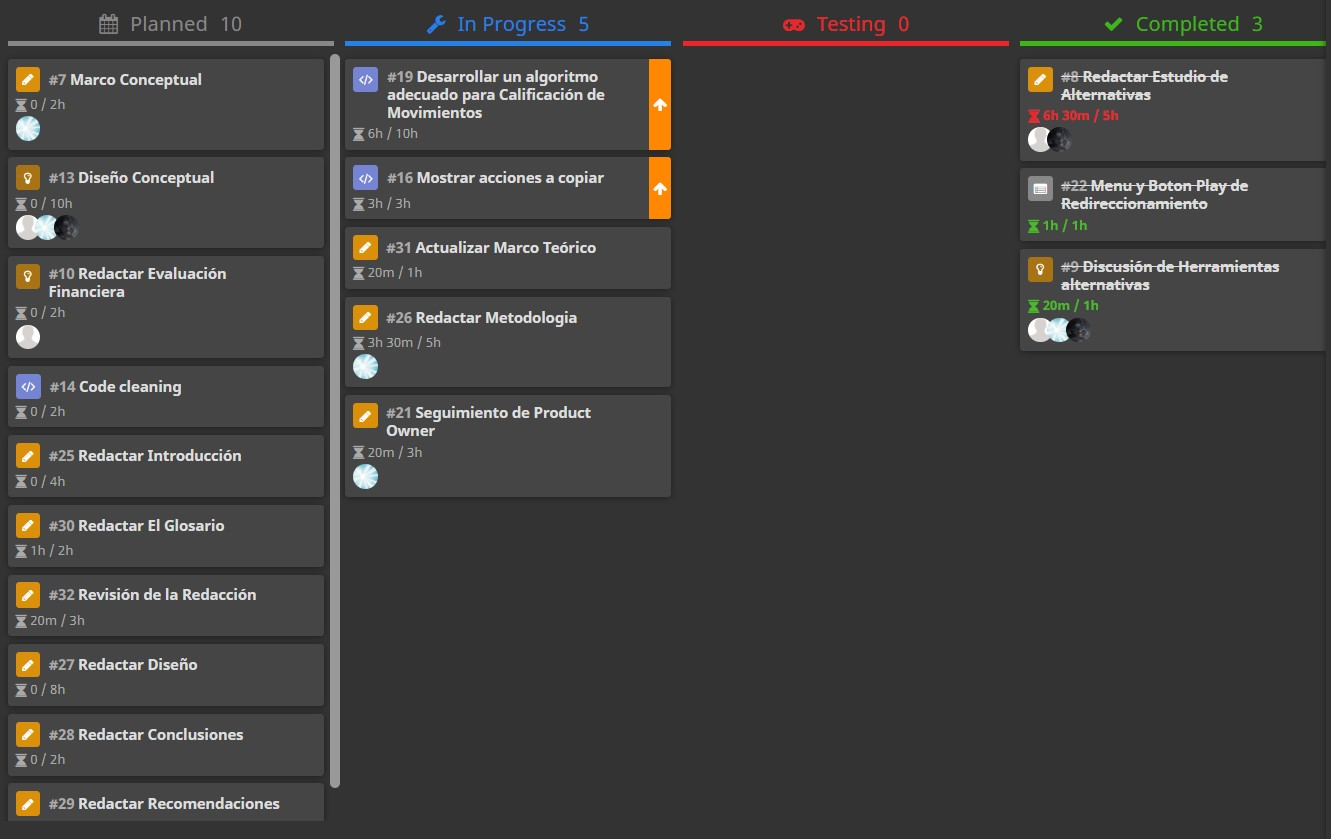
\includegraphics[width=23cm,height=15cm,]{./Images/hacknplanexample.jpg}
	\caption{Sprint Backlog del día 5 de Noviembre}
	\footnotesize Fuente: Elaboración Propia empleando la herramienta HacknPlan.
	\label{sprintexample}
\end{figure}

\end{landscape}

\begin{figure}[t!]
	\centering
	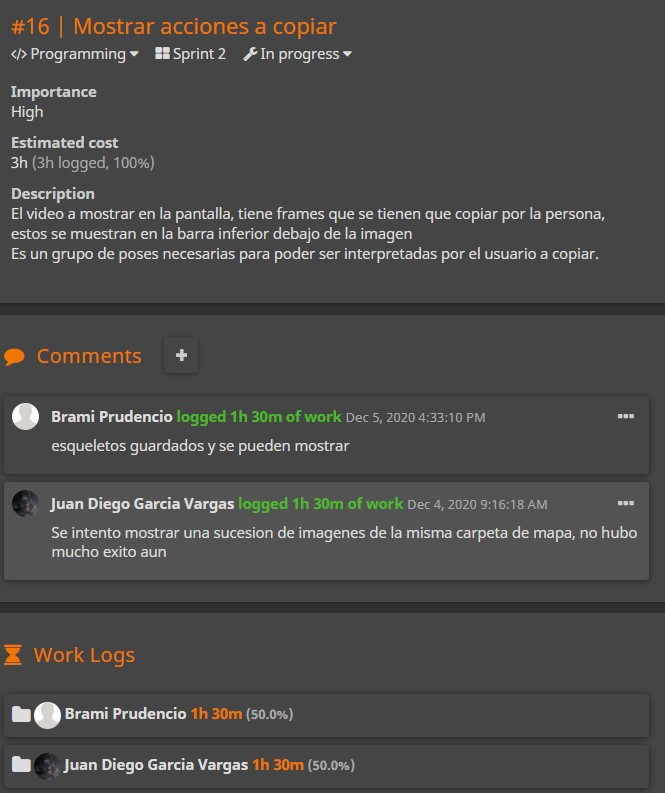
\includegraphics[width=15cm,height=20cm,]{./Images/tareaexample.jpg}
	\caption{Tarea de la Sprint 2, Mostrar Acciones a Copiar}
	\footnotesize Fuente: Elaboración Propia empleando la herramienta HacknPlan.
	\label{sprinttarea}
\end{figure}




